%%%%%%%%%%%%%%%%%%%%%%%%%%%%%%%%%%%%%%%%%
% Journal Article
% LaTeX Template
% Version 1.4 (15/5/16)
%
% This template has been downloaded from:
% http://www.LaTeXTemplates.com
%
% Original author:
% Frits Wenneker (http://www.howtotex.com) with extensive modifications by
% Vel (vel@LaTeXTemplates.com)
%
% License:
% CC BY-NC-SA 3.0 (http://creativecommons.org/licenses/by-nc-sa/3.0/)
%
%%%%%%%%%%%%%%%%%%%%%%%%%%%%%%%%%%%%%%%%%

%----------------------------------------------------------------------------------------
%	PACKAGES AND OTHER DOCUMENT CONFIGURATIONS
%----------------------------------------------------------------------------------------

\documentclass[twoside,twocolumn]{article}

\usepackage{blindtext} % Package to generate dummy text throughout this template 

\usepackage[sc]{mathpazo} % Use the Palatino font
\usepackage[T1]{fontenc} % Use 8-bit encoding that has 256 glyphs
\linespread{1.05} % Line spacing - Palatino needs more space between lines
\usepackage{microtype} % Slightly tweak font spacing for aesthetics

\usepackage[english]{babel} % Language hyphenation and typographical rules

\usepackage[hmarginratio=1:1,top=32mm,columnsep=20pt]{geometry} % Document margins
\usepackage[hang, small,labelfont=bf,up,textfont=it,up]{caption} % Custom captions under/above floats in tables or figures
\usepackage{booktabs} % Horizontal rules in tables

\usepackage{lettrine} % The lettrine is the first enlarged letter at the beginning of the text

\usepackage{enumitem} % Customized lists
\setlist[itemize]{noitemsep} % Make itemize lists more compact

\usepackage{abstract} % Allows abstract customization
\renewcommand{\abstractnamefont}{\normalfont\bfseries} % Set the "Abstract" text to bold
\renewcommand{\abstracttextfont}{\normalfont\small\itshape} % Set the abstract itself to small italic text

\usepackage{titlesec} % Allows customization of titles
\renewcommand\thesection{\Roman{section}} % Roman numerals for the sections
\renewcommand\thesubsection{\roman{subsection}} % roman numerals for subsections
\titleformat{\section}[block]{\large\scshape\centering}{\thesection.}{1em}{} % Change the look of the section titles
\titleformat{\subsection}[block]{\large}{\thesubsection.}{1em}{} % Change the look of the section titles

\usepackage{fancyhdr} % Headers and footers
\pagestyle{fancy} % All pages have headers and footers
\fancyhead{} % Blank out the default header
\fancyfoot{} % Blank out the default footer
\fancyhead[C]{Running title $\bullet$ May 2016 $\bullet$ Vol. XXI, No. 1} % Custom header text
\fancyfoot[RO,LE]{\thepage} % Custom footer text

\usepackage{titling} % Customizing the title section

\usepackage{hyperref} % For hyperlinks in the PDF

\usepackage{graphicx}

%----------------------------------------------------------------------------------------
%	TITLE SECTION
%----------------------------------------------------------------------------------------

\setlength{\droptitle}{-4\baselineskip} % Move the title up

\pretitle{\begin{center}\Huge\bfseries} % Article title formatting
\posttitle{\end{center}} % Article title closing formatting
\title{Report on the evolution of cooperation in relation to game-theory and different game-theoretic mechanisms to aid it} % Article title
\author{%
\textsc{James King} \\% Your name
\normalsize Supervisor: Kostas Stathis \\ % Your supervisor
}
\date{October 2018} % Leave empty to omit a date
\renewcommand{\maketitlehookd}{%
\begin{abstract}
\noindent Since the early days of Darwinian evolutionary theory the phrase ``Survival of the fittest" has become synonymous with much thinking on evolutionary dynamics. This idea has come along way since then but is still seen by many to promote selfish attitudes. However, we can see throughout nature that cooperation between biological agents is prevalent. So how did cooperation evolve and why has it flourished? This question fundamentally challenges what seemed concrete ideas about evolutionary dynamics, and has been approached from many angles. Game-theory is a branch of mathematics that has spawned many mathematical models of evolutionary dynamics in an attempt to solve the problem, some have been formulated programmatically to analyse the results. Study of the evolution of cooperation also has wider impacts in the world of computer science - namely on agent-based systems. A large component of agent-based system design is how interactions between agents works and how cooperation can be garnered within societies of agents. In this report, I shall explore past game-theoretic approaches to this problem. This exploration will help me gather a deeper understanding of evolutionary dynamics and the reasoning behind these mathematical approaches to the problem of the evolution of cooperation.
\end{abstract}
}

%----------------------------------------------------------------------------------------

\begin{document}

% Milestone: Report on the evolution of cooperation in relation to game-theory and different game-theoretic mechanisms to aid it
% Report on past work in this area such as Axelrod’s tournaments [1] and Nowak’s five rules for the evolution of cooperation [4].
% Link to goal: This will act as a starting point for my exploration of the mechanisms for the evolution of cooperation and help motivate the implementation of the web application.


% Print the title
\maketitle

%----------------------------------------------------------------------------------------
%	ARTICLE CONTENTS
%----------------------------------------------------------------------------------------

\section{Introduction}
In the seminal paper on the evolution of cooperation~\cite{evolution_of_cooperation} Axelrod and Hamilton highlighted the failure of past ideas on Darwinian evolutionary theory to account for altruistic behaviour. Their paper identifies two theories proposed to solve the problem: kinship theory and reciprocation theory, focusing on the latter - particularly the Iterated Prisoner's Dilemma.\\ 
Altruistic acts are actions where an individual puts others above themselves, meaning that they act in a way that benefits others and is detrimental in some way to themselves. The proposed theories attempt to explain how altruistic behaviours have evolved in our world.\\
Here I will explore these mechanisms that attempt to explain altruistic behaviour and attempt to relate them to multi-agent systems or even point out how they are inapplicable to this domain if appropriate.\\

%------------------------------------------------

\section{Content and Knowledge}
\subsection{Kinship Theory}
Kinship theory is an umbrella term for a number of theories that attempt tp solve the problem of the evolution of cooperation. The tie between these theories is that the individuals who choose to cooperate with each other are in some way `kin'. The definition of what `kin' is varies depending on the theory and the purpose for that theory.\\
Richard Dawkins popularized the idea of the `selfish gene'~\cite{selfish_gene}. This `selfish gene' idea argues that as genes are the actual replicators, actors are hardwired to have a will to propagate the gene. This propagation does not only involve reproduction but also acts of cooperation to support and maintain others who share the gene. This is evident in many areas of nature especially in the family groups of different species, shown even recently in the BBC series Dynasties.\\
W.D. Hamilton supports a similar view~\cite{kinhamilton}: that agents with shared genes will work together to preserve those genes. He argues that to do this individuals don't work to add to their own fitness, but work to improve their `inclusive fitness', which includes the fitness of other related individuals. His model converts the extent of the relatedness of an individual to a quantitative value using Wright's Coefficient of Relationship, which is shown in figure~\ref{fig:coefrelate} on page~\pageref{fig:coefrelate}. The model then uses this coefficient of relatedness to calculate inclusive fitness.\\
\begin{figure}
	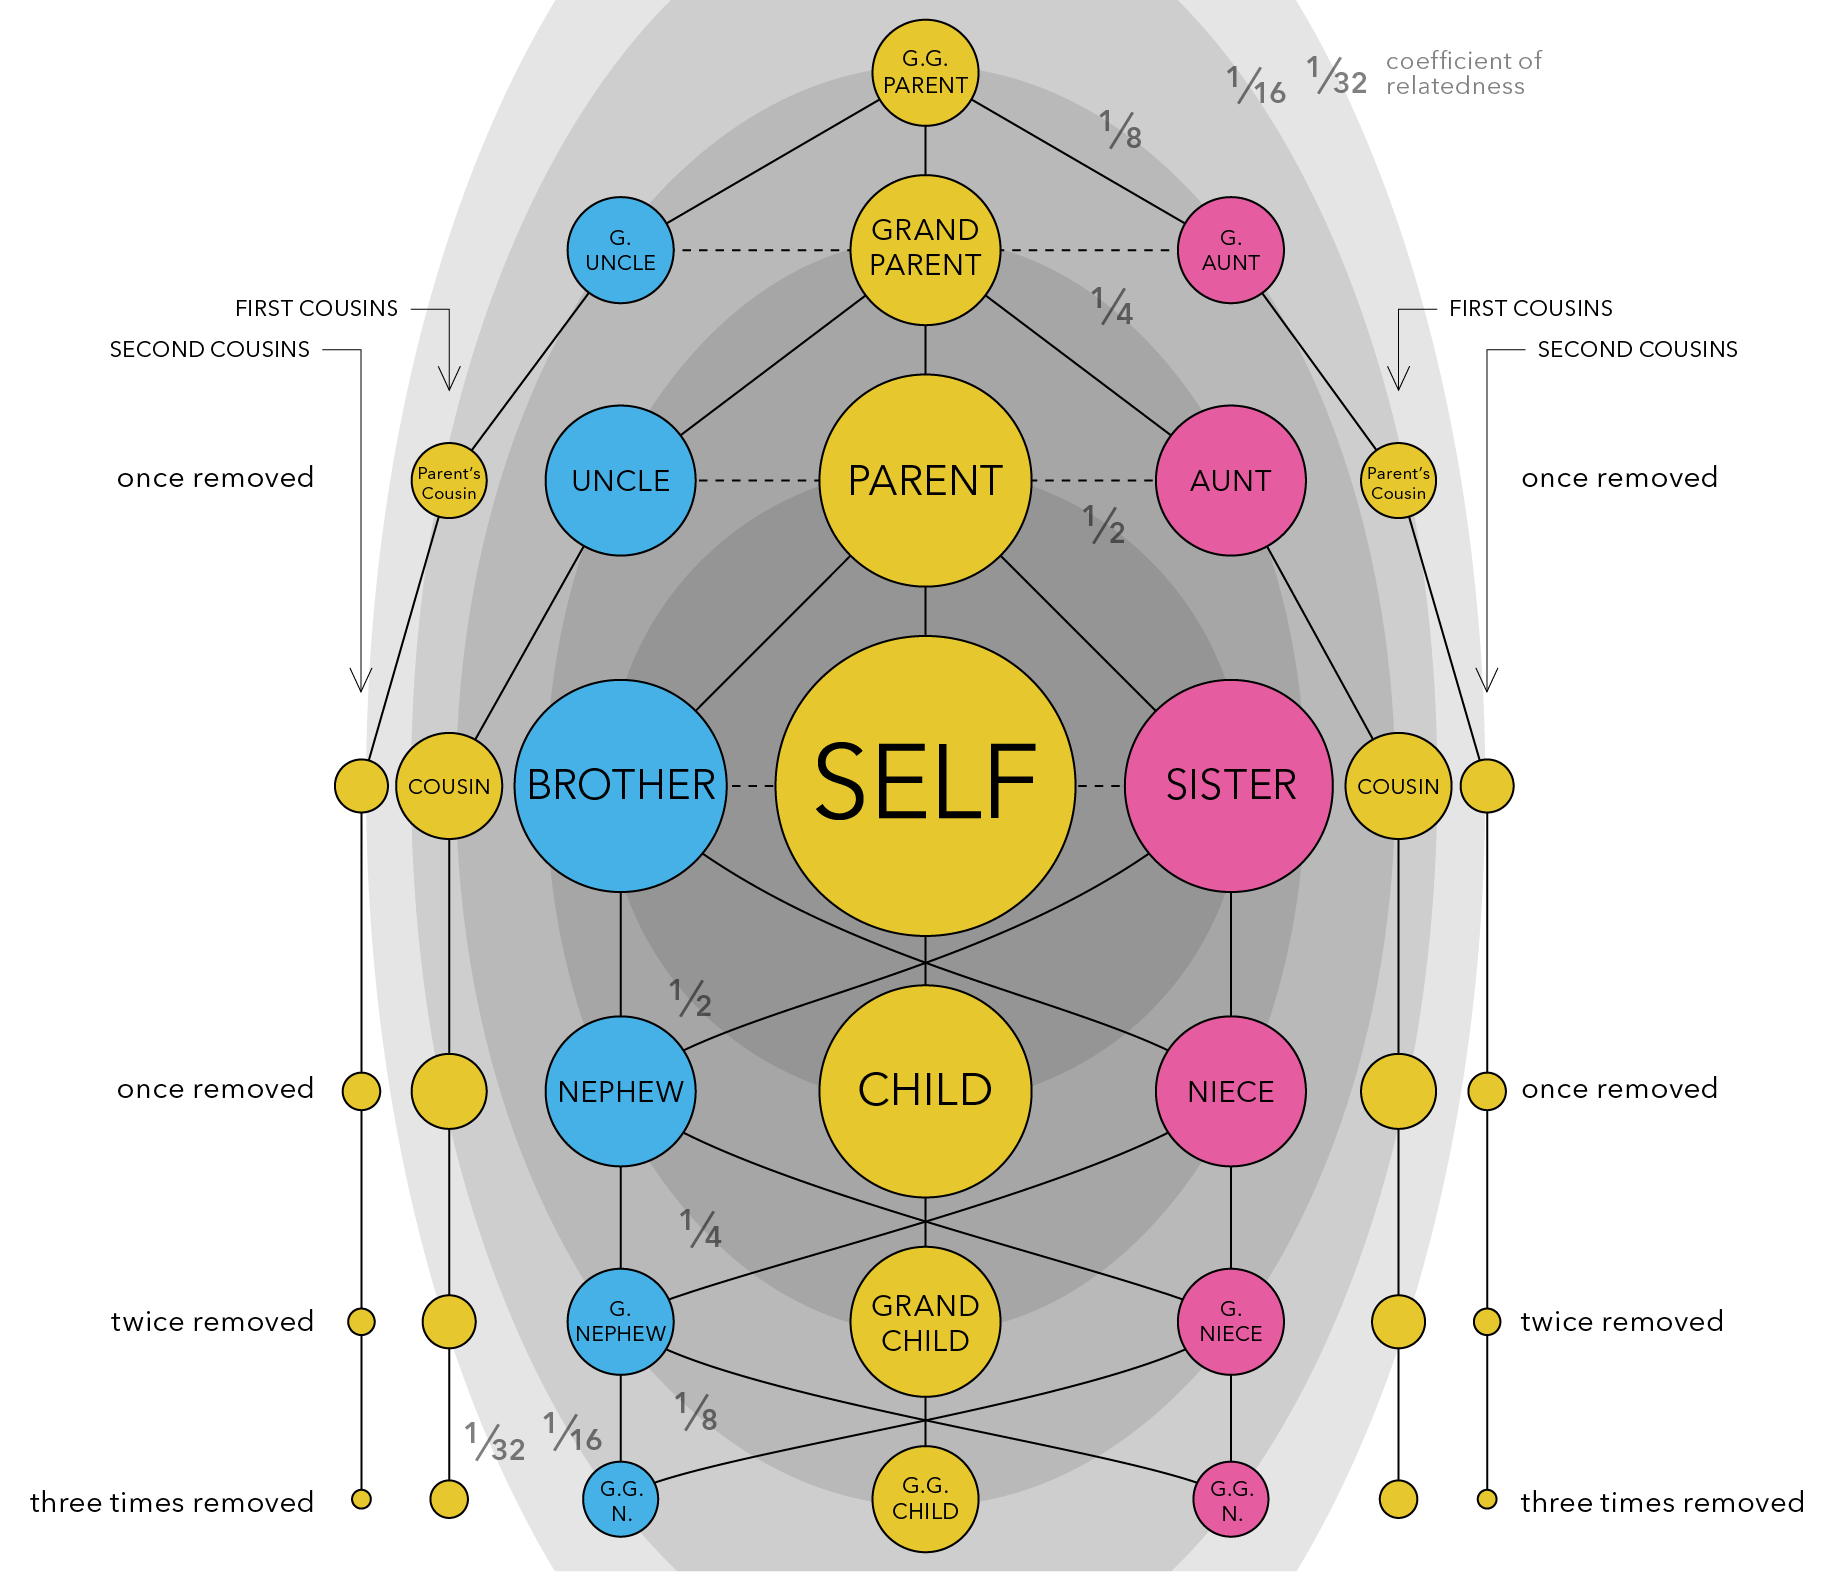
\includegraphics[width=0.5\textwidth]{coefrelate.png}
	\caption{By Citynoise - Own work, CC BY-SA 4.0, \url{https://commons.wikimedia.org/w/index.php?curid=37723128}}
	\label{fig:coefrelate}
\end{figure}
Axelrod and Hamilton~\cite{evolution_of_cooperation} highlight that although the theory works well to explain cooperation between related individual it falls short in explaining the evolution of cooperation between unrelated individuals. This also makes it difficult to apply kinship theory as an aid to the evolution of cooperation in multi-agent systems. Kinship theory requires a reproductive drive and metrics for relatedness in order to motivate altruistic acts, both of which would likely be missing in a decentralised multi-agent system.

\subsection{The Iterated Prisoner's Dilemma}
The Iterated Prisoner's Dilemma is one such example of a game-theoretic model that uses direct reciprocity to attempt to solve the problem that the evolution of cooperation puts forward. Direct reciprocity is the idea: ``If I cooperate now, you may cooperate later''~\cite{five_rules_coop}. The Dilemma is in fact a game played between two individuals. The game is made up of a number of repeated rounds, in each round the two players can choose between cooperating with or defecting against each other.\\
A payoff matrix is provided such as the one in figure~\ref{fig:payoffmatrix} on page~\pageref{fig:payoffmatrix}. These matrices provide a temptation to defect, but a reward if both players cooperate over multiple rounds. In a single round game it is mathematically best to defect, but in repeated rounds agents are encouraged to cooperate by a mutual gain in payoff. These payoffs attempt to simulate resource gains from interactions in real life.\\
The dilemma has been extended into tournaments such as the one in Axelrod and Hamilton~\cite{evolution_of_cooperation}. You can even run tournaments directly in Python using the Axelrod-Python library~\cite{axelrodproject}. Tournaments can come in a variety of styles but the most popular is the round-robin tournament where every player plays a match of the iterated prisoner's dilemma against every other player. Players accumulate points throughout these games, based on the payoff matrix.\\
This has been even further extended to include a genetic algorithm to simulate evolution by reproducing players into a next generation. Multiple different algorithms have been used, one common one is the Moran Process (A stochastic process used to model evolution in a finite, unstructured population) available in the Axelrod-Python library. 
\begin{figure}
	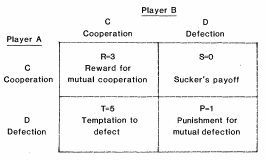
\includegraphics[width=0.5\textwidth]{payoffmatrix.png}
	\caption{The payoff matrix given in Axelrod and Hamilton's paper~\cite{evolution_of_cooperation}}
	\label{fig:payoffmatrix}
\end{figure}
\subsection{Strategies}

\subsection{Other Reciprocation Theories}



~\cite{arithmetics_of_mutual_help}\\
~\cite{five_rules_coop}\\
~\cite{evolution_of_cooperation}\\
~\cite{evol_indirect_image}\\
~\cite{evol_graph}\\
~\cite{multilevel_nowak}\\
~\cite{phelps_game_theoretic_analysis}\\
~\cite{spatial}\\
~\cite{heterogenous}\\
~\cite{evoldirindir}\\
~\cite{extortion}\\

%------------------------------------------------

\section{Discussion and Conclusion}
Talk about why I am choosing indirect reciprocity.\\
Talk about impact in real life and multi-agent systems.\\
~\cite{sticklebacks}\\
~\cite{prisonersdilemma}\\


%----------------------------------------------------------------------------------------
%	REFERENCE LIST
%----------------------------------------------------------------------------------------

\bibliography{../refs.bib}{}
\bibliographystyle{plain}

%----------------------------------------------------------------------------------------

\end{document}
